\providecommand{\main}{../../../..}
\documentclass[\main/dresen_thesis.tex]{subfiles}
\begin{document}
  \label{sec:colloidalCrystals:layers:sem}

  \begin{figure}[tb]
    \centering
    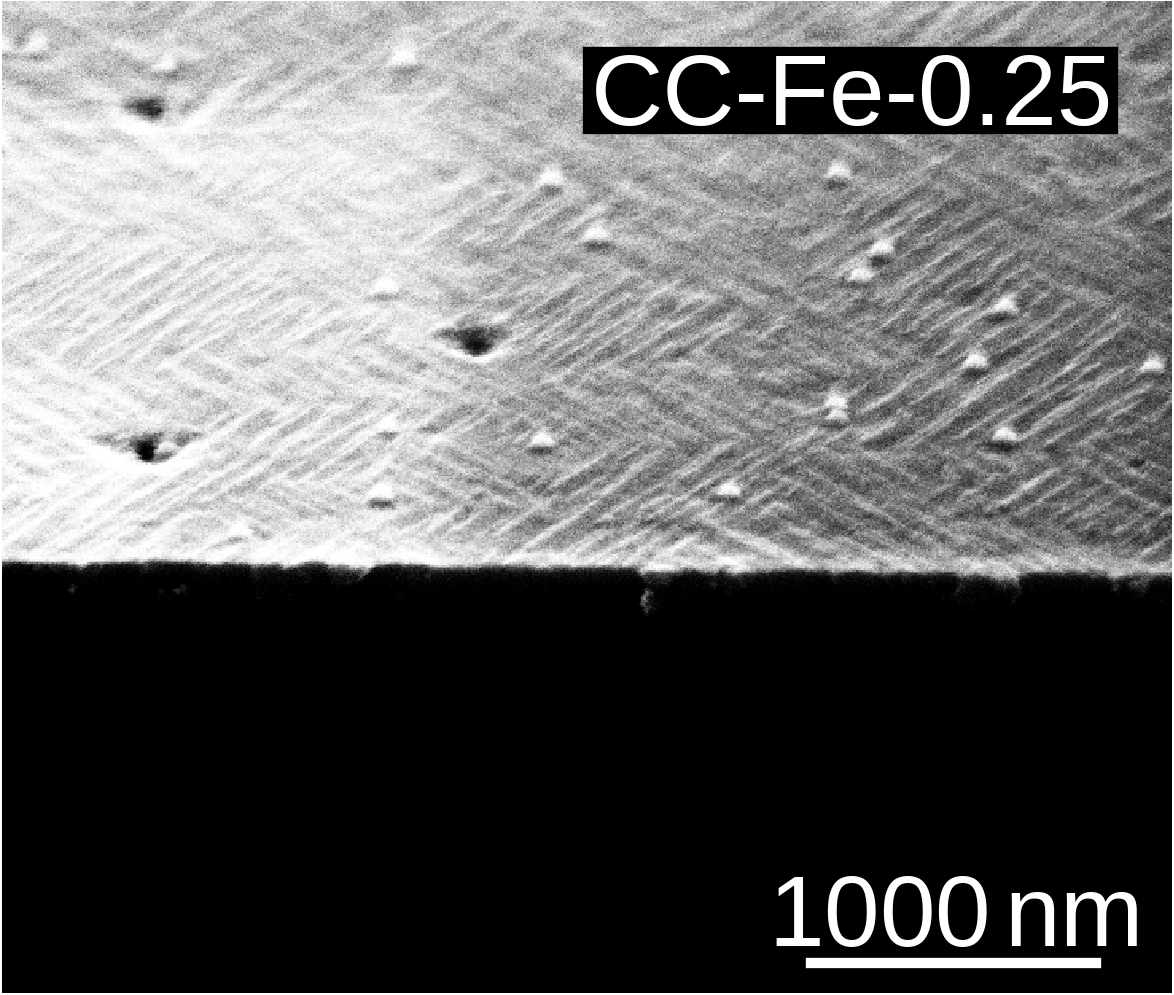
\includegraphics{colloidalCrystals_SEM_CC-Fe-0_25_xsSmallZoom}
    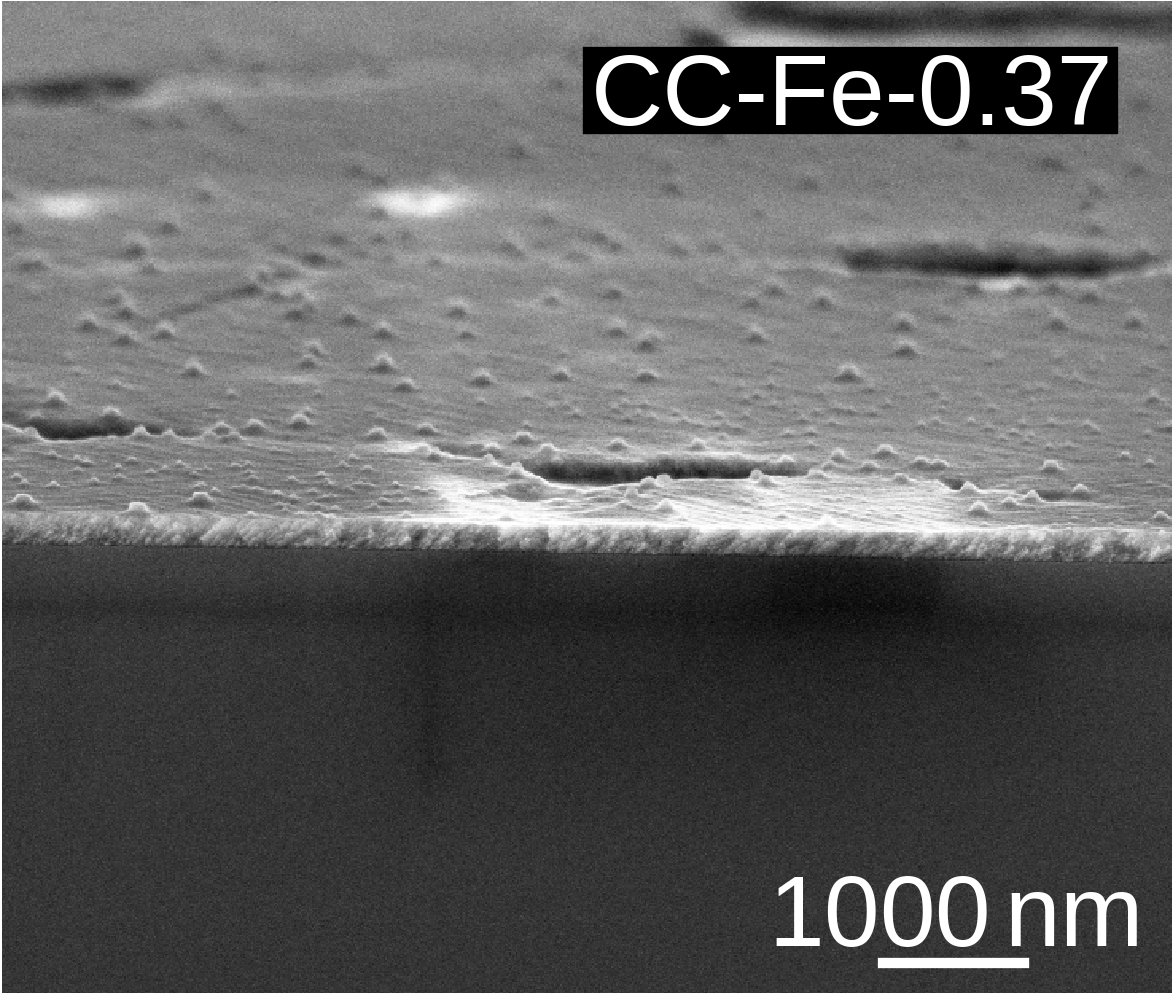
\includegraphics{colloidalCrystals_SEM_CC-Fe-0_37_xsSmallZoom}
    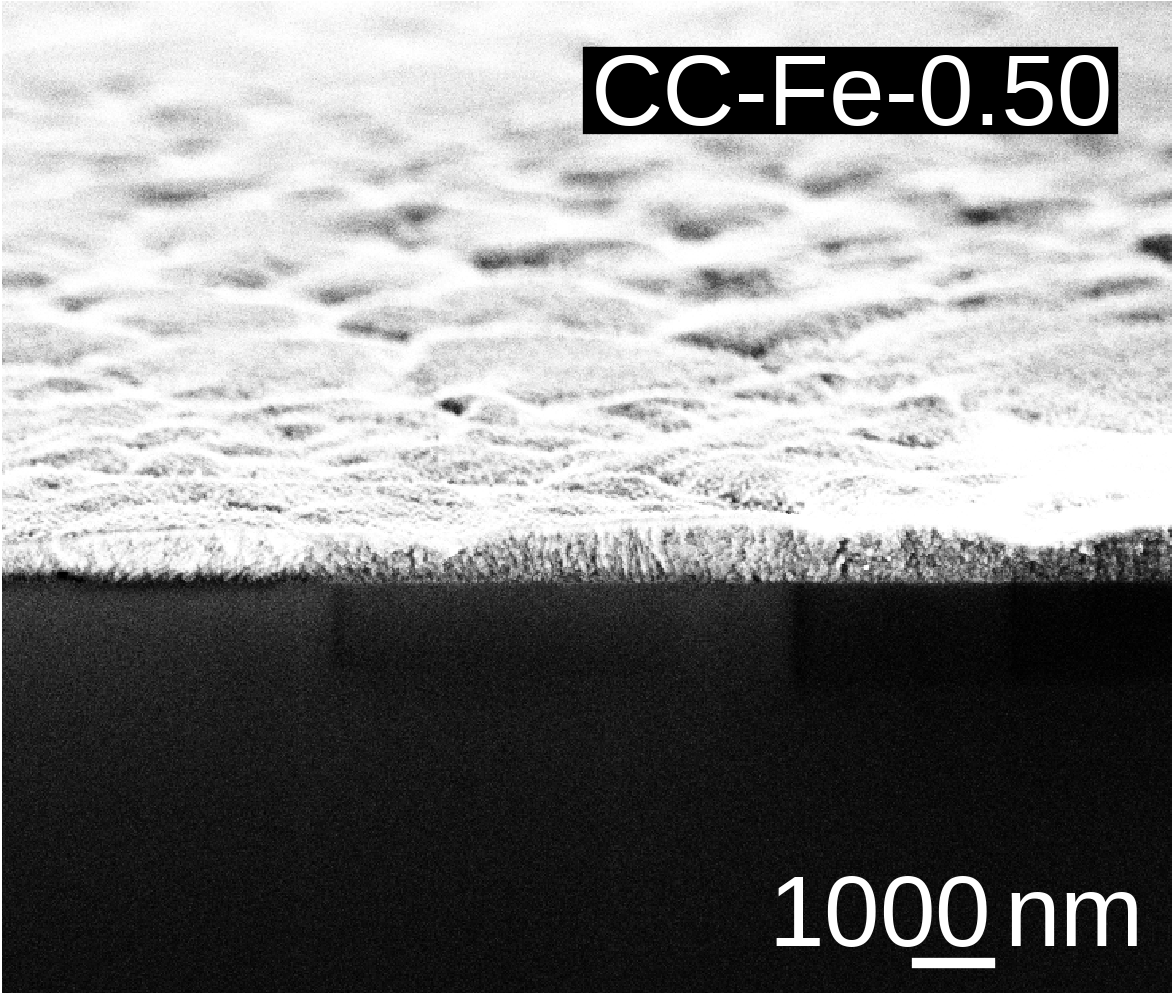
\includegraphics{colloidalCrystals_SEM_CC-Fe-0_50_xsSmallZoom}
    \caption{\label{fig:colloidalCrystals:structure:semLowMag}Cross-sectional micrographs of CC-Fe-0.25 (left), CC-Fe-0.37 (center), CC-Fe-0.50 (right) with low magnification.}
  \end{figure}

  \begin{figure}[tb]
    \centering
    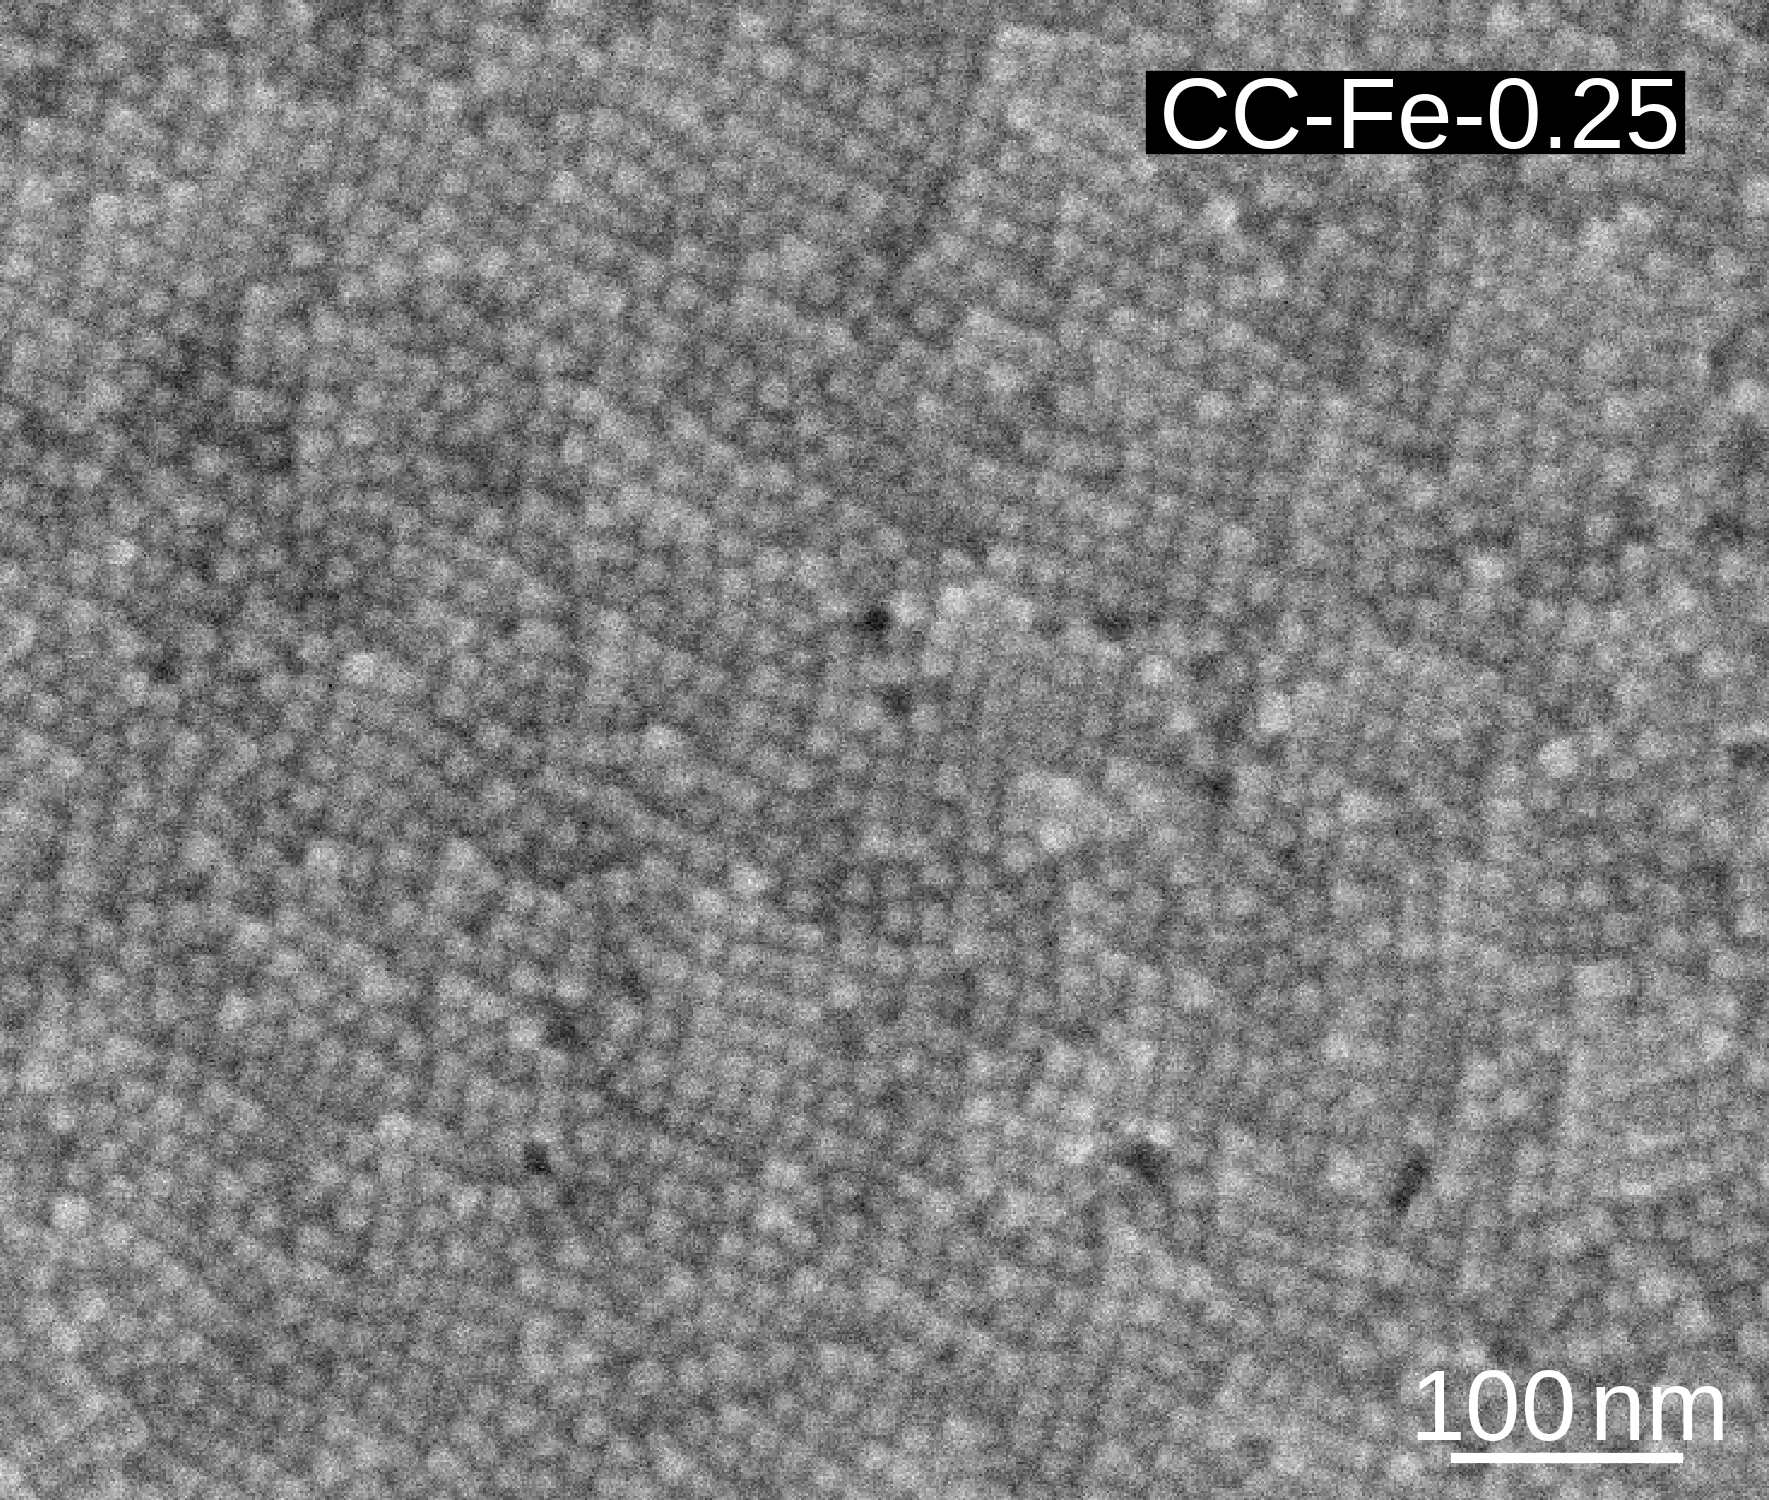
\includegraphics{colloidalCrystals_SEM_CC-Fe-0_25}
    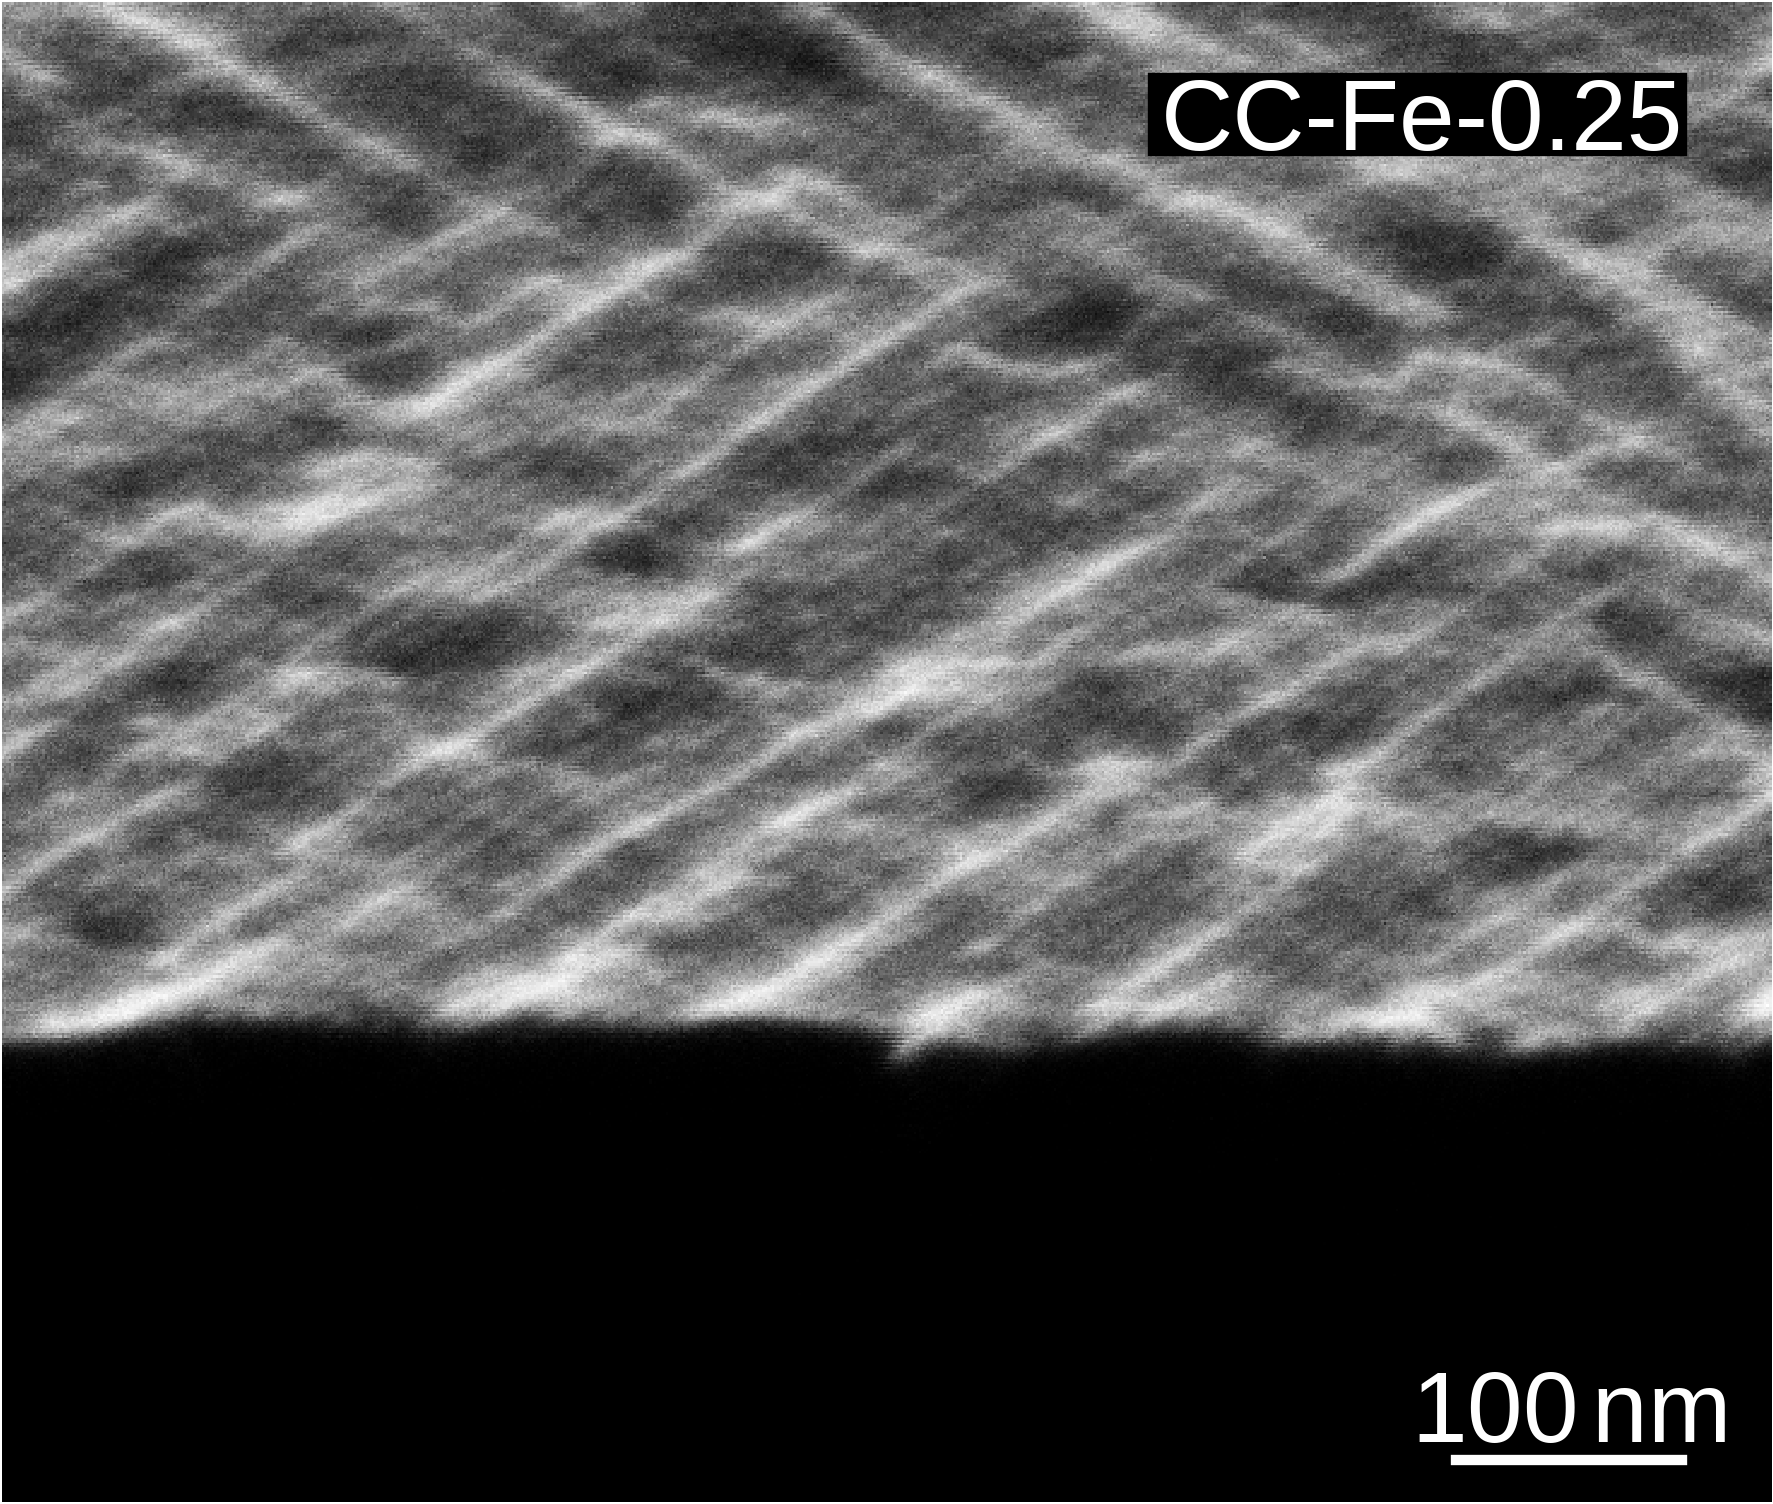
\includegraphics{colloidalCrystals_SEM_CC-Fe-0_25_xs}
    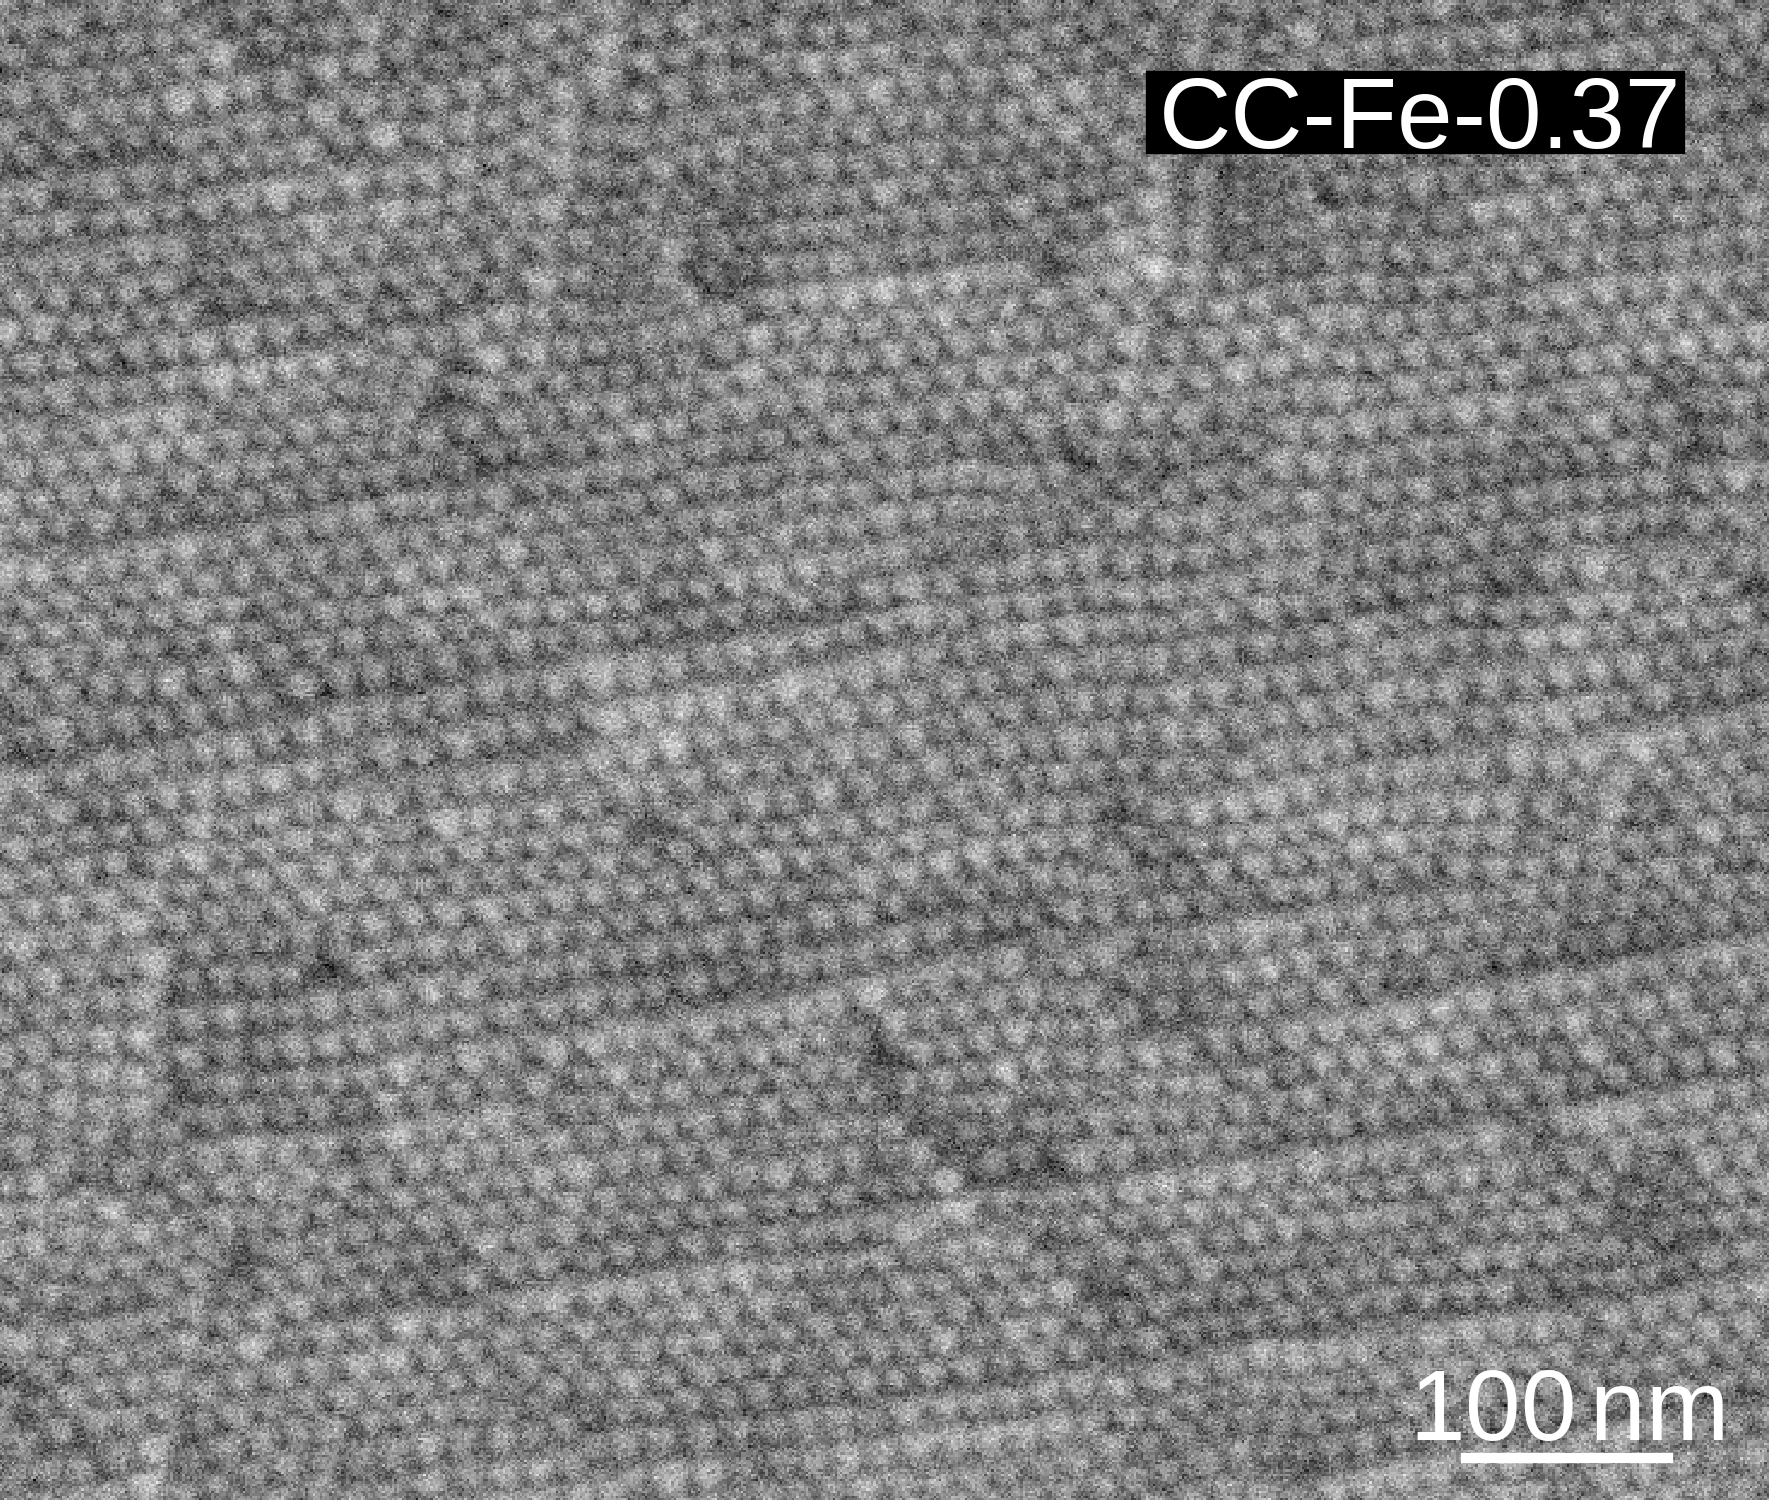
\includegraphics{colloidalCrystals_SEM_CC-Fe-0_37}
    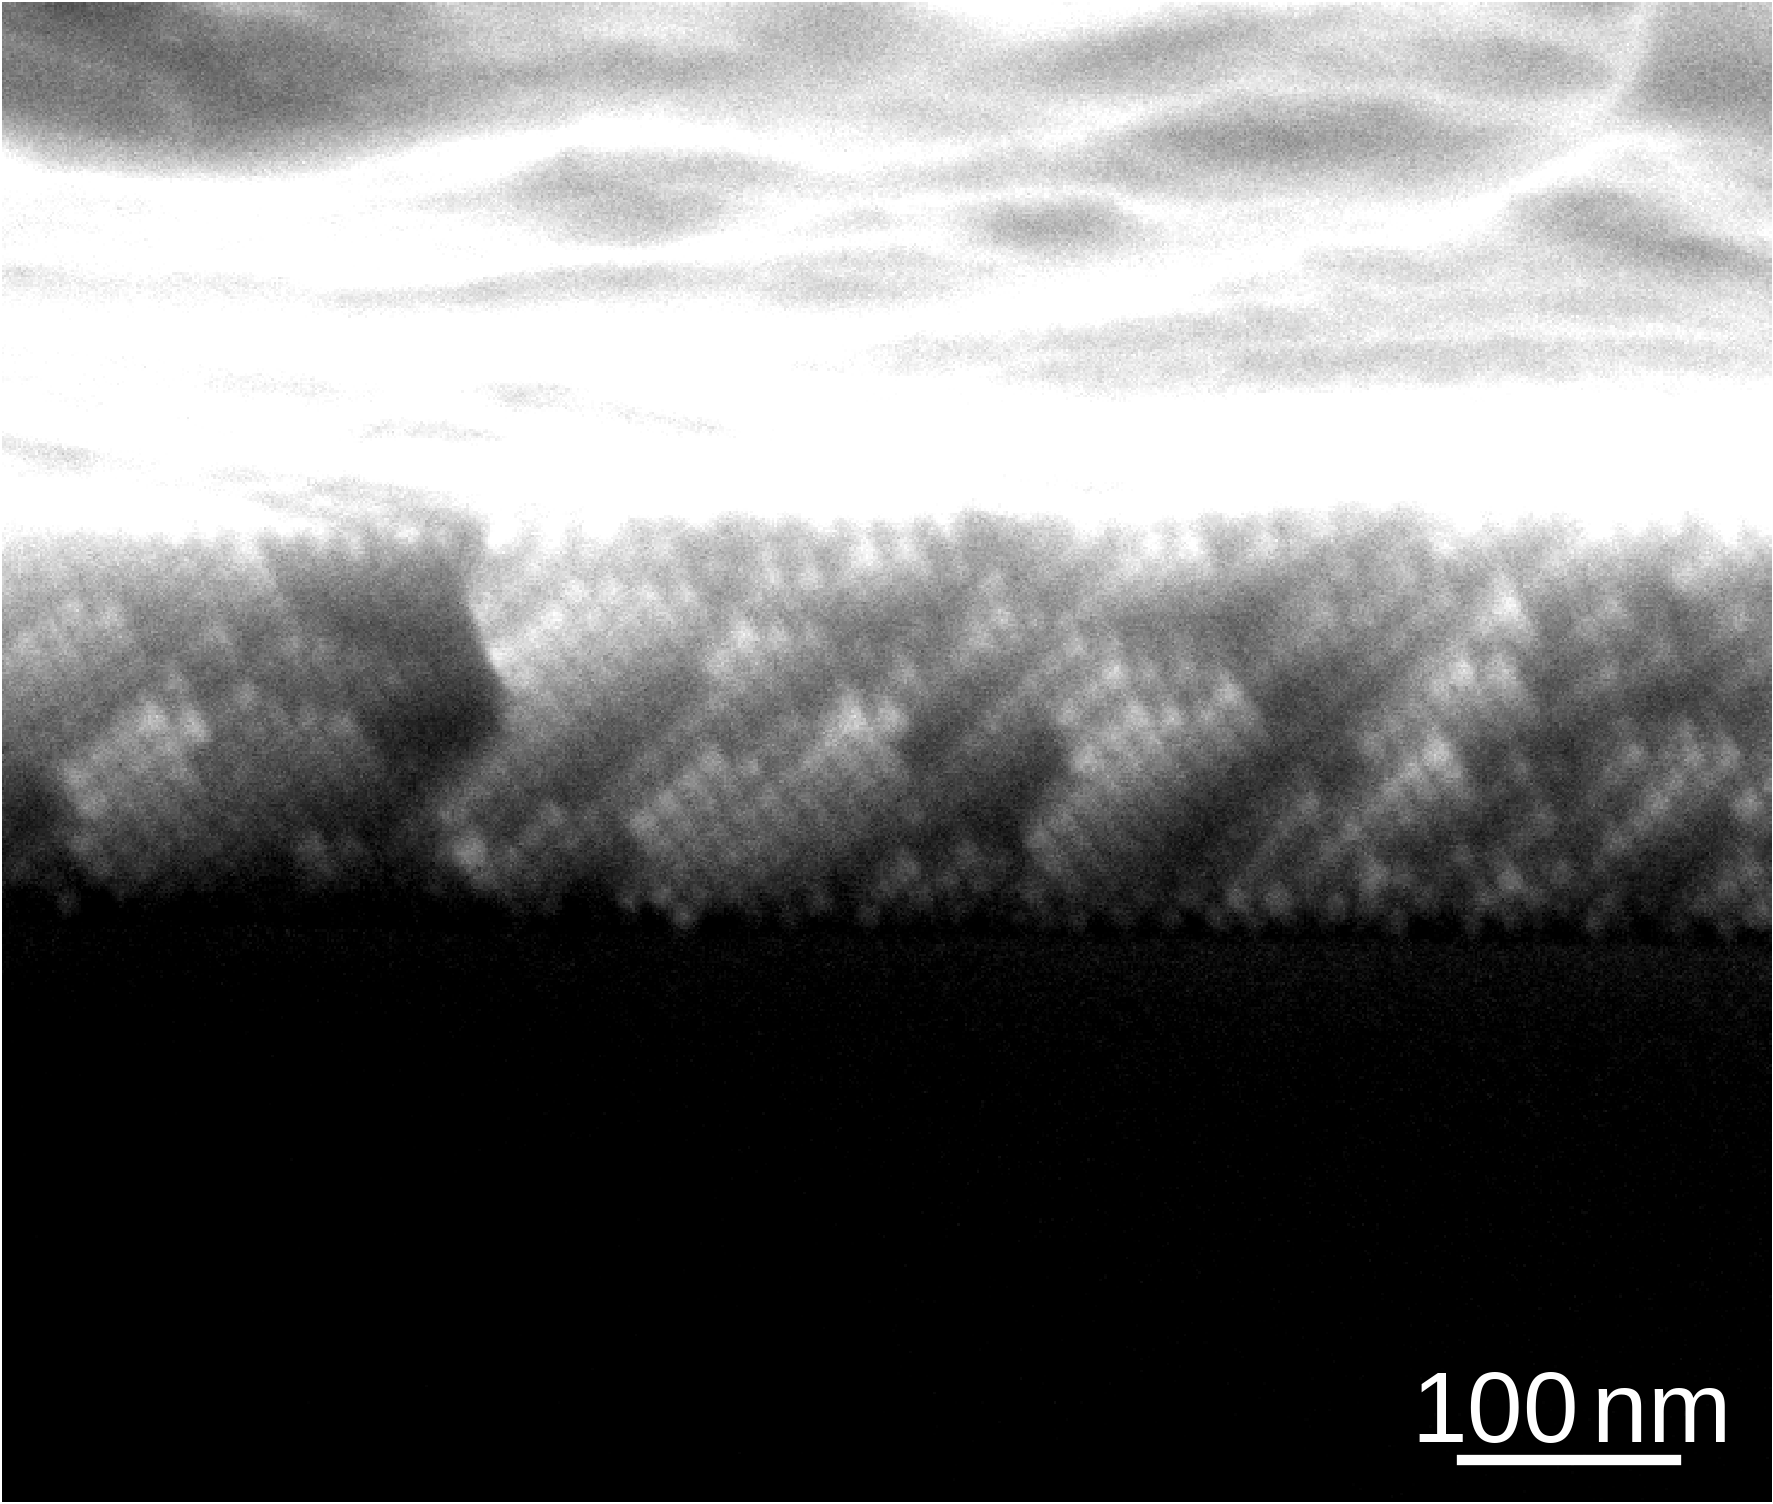
\includegraphics{colloidalCrystals_SEM_CC-Fe-0_37_xs}
    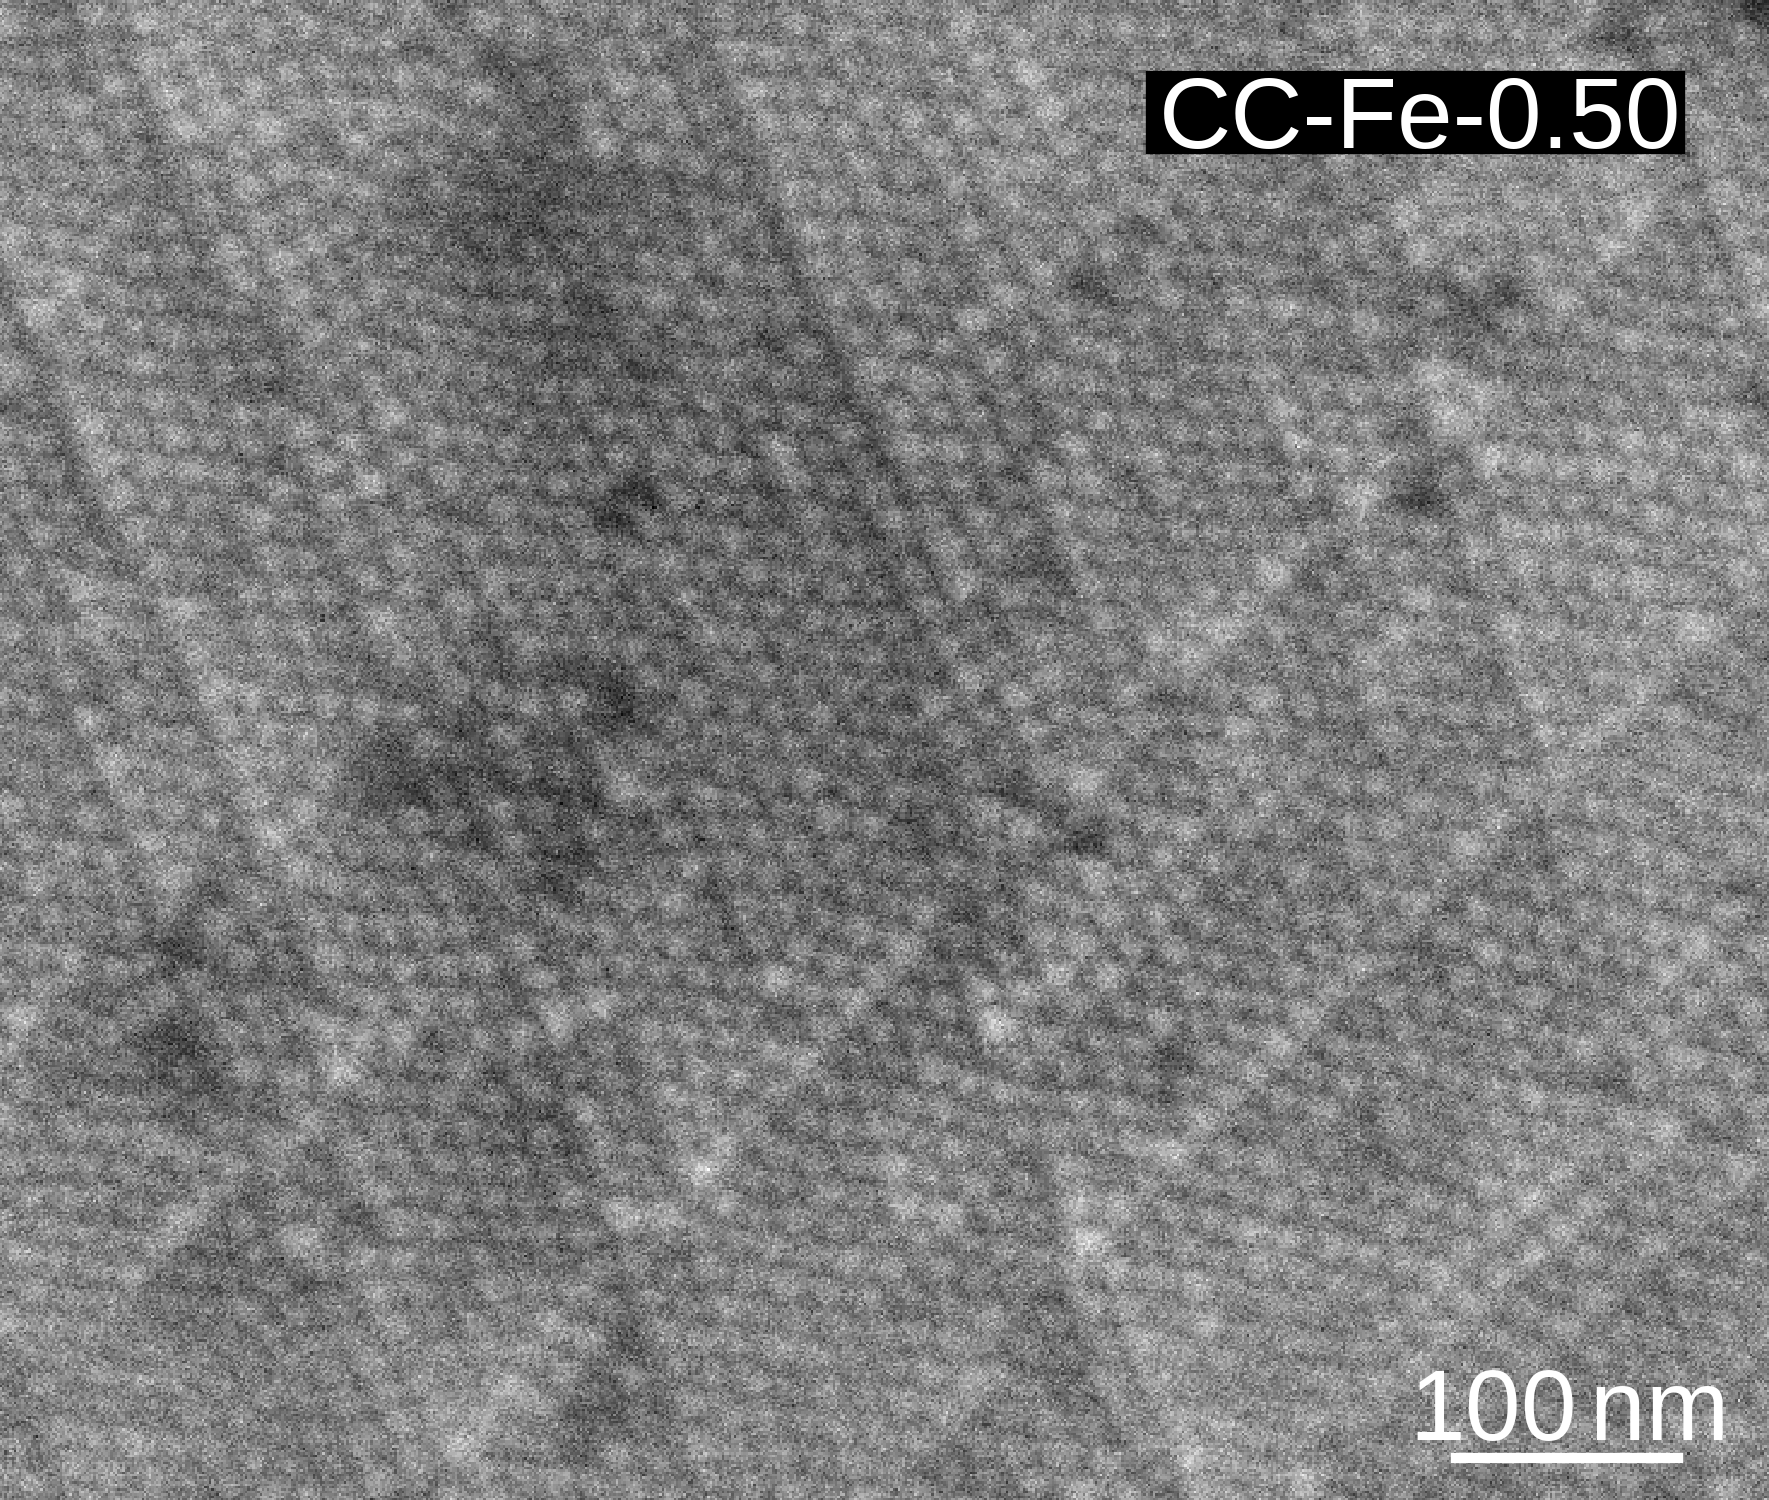
\includegraphics{colloidalCrystals_SEM_CC-Fe-0_50}
    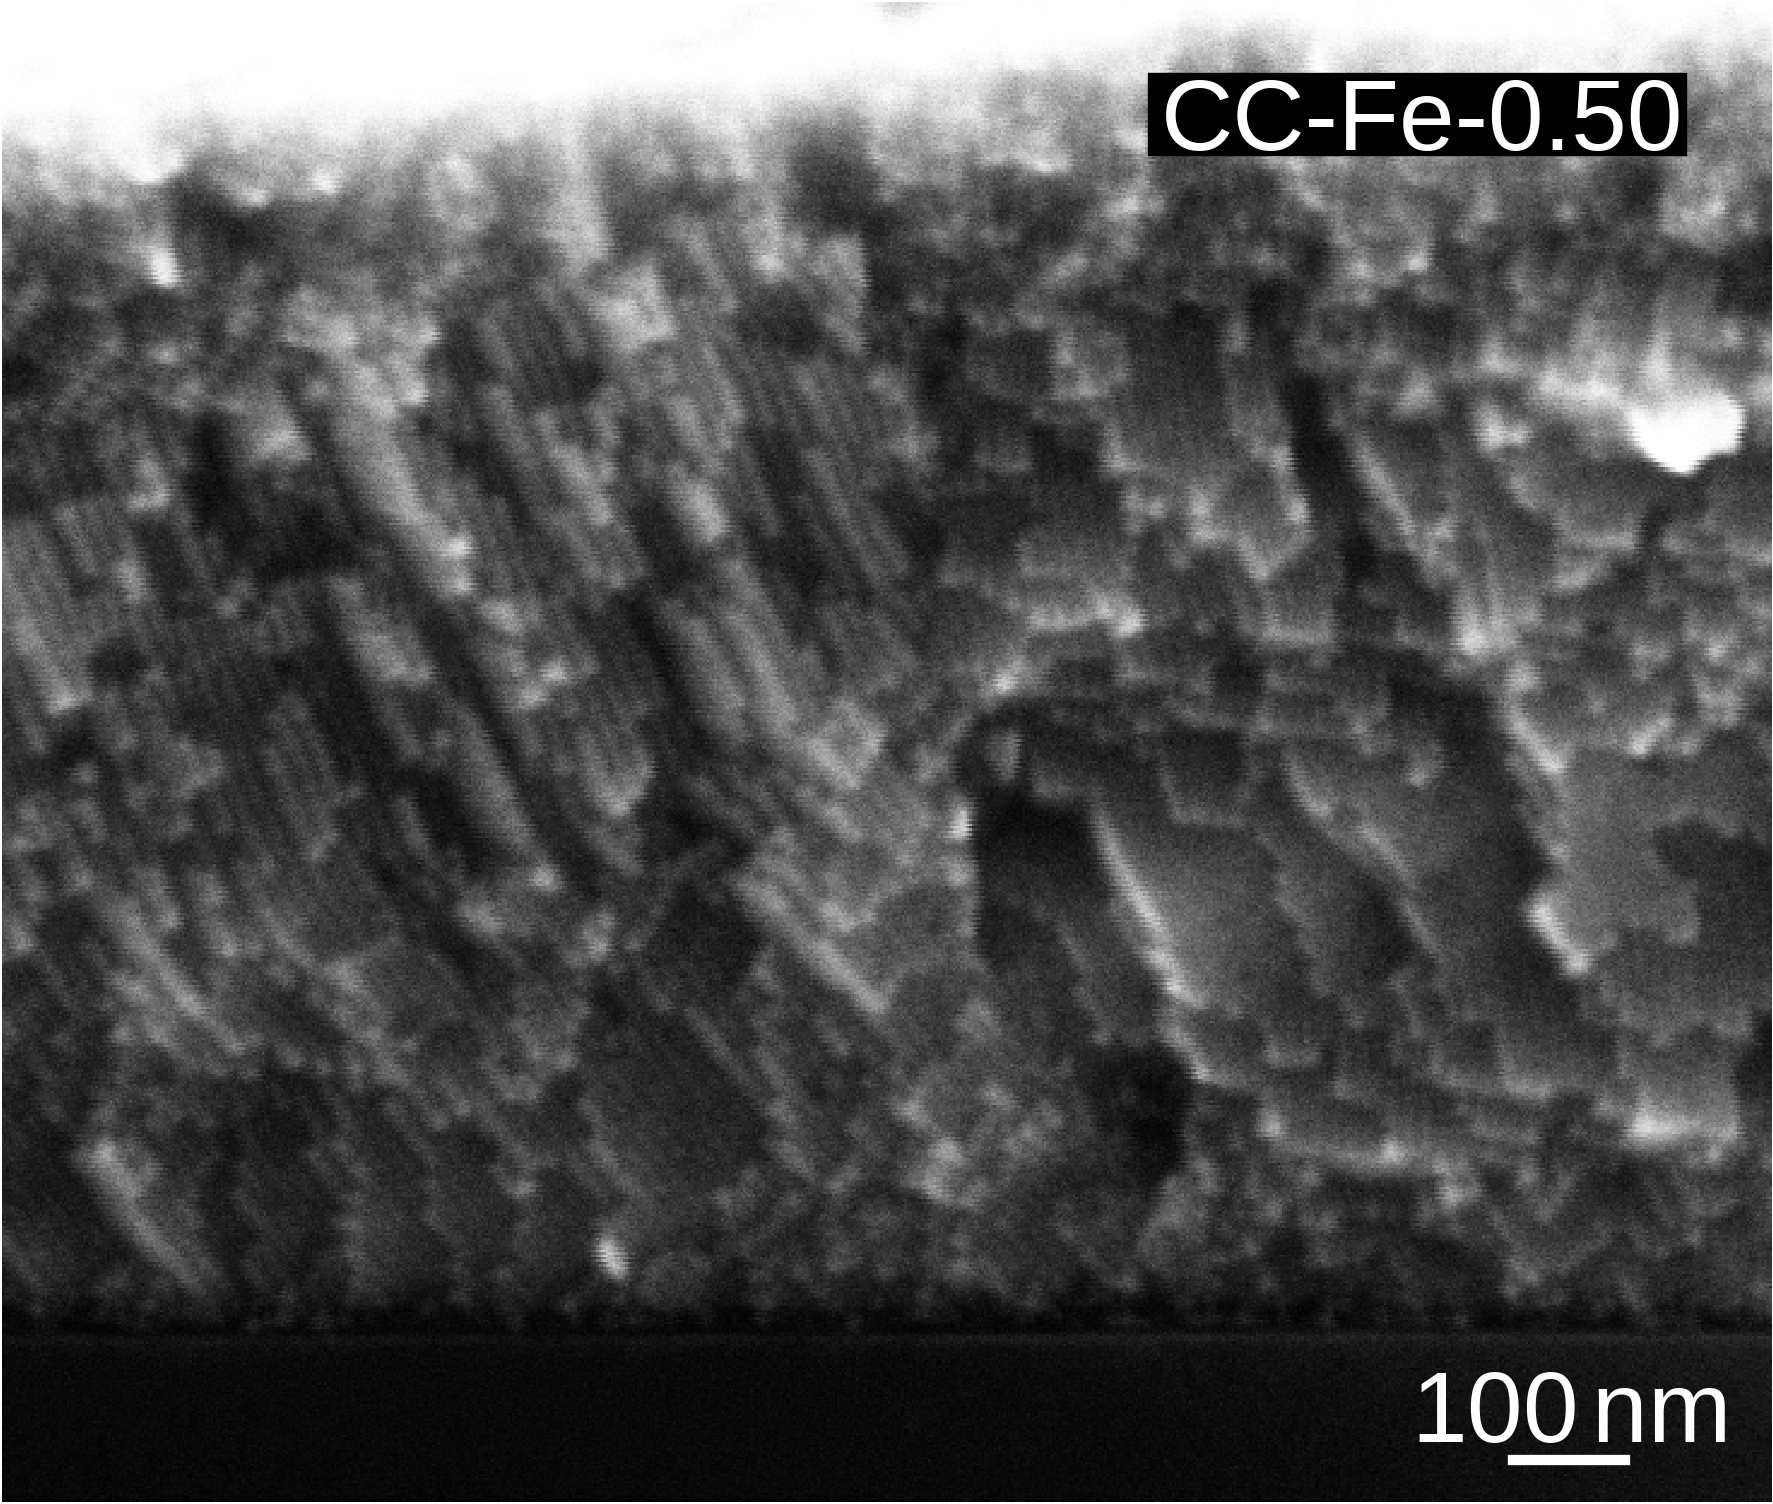
\includegraphics{colloidalCrystals_SEM_CC-Fe-0_50_xs}
    \caption{\label{fig:colloidalCrystals:structure:sem}Micrographs CC-Fe-0.25 (upper), CC-Fe-0.37 (center), CC-Fe-0.50 (lower) viewed from the top (left) and a cross-sectional view (right). }
  \end{figure}
  Using scanning electron microscopy the structure of the colloidal crystals is probed at multiple positions of the sample, where exemplary top views and cross-sectional micrographs are shown in \reffig{fig:colloidalCrystals:structure:sem}.
  From the cross-sectional views it is visible that by variation of the nanoparticle concentration in the dispersion, the crystal thickness is non-linearly tuned.
  Where the dispersion with $0.25 \unit{mg \, mL^{-1}}$ shows only a thin layer of ordered cubes, $0.50 \unit{mg \, mL^{-1}}$ leads to a thickness close to a micrometer.

  From lower magnification views of the cross-section, shown in \reffig{fig:colloidalCrystals:structure:semLowMag}, a relatively homogeneous thickness is observed for CC-Fe-0.25 and CC-Fe-0.37, but a high variation in thickness in CC-Fe-0.50.
  All samples show holes in the structure and organic remnants are visible on the surface of CC-Fe-0.25 and CC-Fe-0.37.
  The holes in the structures suggest an incomplete wetting of wafer surface during the vertical evaporation, which resulted in the formation of empty spots in the structure.

  From the top view micrographs, the formation of terraces on the sample surface that stretch over several $100 \unit{nm}$ is visible.
  The best ordering in the cross-sectional view is observed for CC-Fe-0.37, where for CC-Fe-0.25 the sample is not thick enough to evaluate the vertical ordering.
  For CC-Fe-0.50 the more disordered structure could be due to the violent breaking of the thick sample that is necessary to obtain cross-sectional SEM.
  However, the thickness variation visible in the low magnification view of \reffig{fig:colloidalCrystals:structure:semLowMag} suggests a large structural variation across the sample.


  % By using scanning electron microscopy, micrographs of the local structure are obtained for both SC-IOS-11  and SC-IOS-7 in \reffig{fig:looselyPackedNP:nuclearStructure:sem}.
  % At close inspection of the top view, voids can be seen in both structures, which alludes to a loose packing of the spheres.
  % Furthermore, the top view shows no long range order among the nanoparticles.

  % The cross-sectional view shows in both cases a relative homogeneous layer of nanospheres with only a low surface roughness.
  % The low surface roughness of the samples is expected for a spin-coated sample and is also a prerequisite to be able to study the sample quantitatively with reflectometry experiments in the following.
  % The thickness of the layer is estimated from the cross-sectional images to $65 \unit{nm}$ for SC-IOS-11 and $55 \unit{nm}$ for SC-IOS-7.

  % Spheres that do not undergo any ordering process and are packed randomly have been studied extensively on the macroscopic scale \cite{Torquato_2000_IsRan} and it has been shown experimentally that the densest random close packing (RCP) lies in the order of $\approx 64 \, \%$.
  % In a long range ordered crystalline structure, the closest packing spheres can achieve are the face-centered cubic and the hexagonal close-packed structure, which have a packing of $74 \, \%$.
  % To study the packing of the nanoparticles, X-ray and neutron scattering provide non-destructive tools to quantify the order of the volume fraction across a large area of the sample.
  % X-ray and neutron reflectometry is used to study the vertical structure of the sample, and grazing incidence small-angle X-ray scattering to study the lateral structure.

  % \begin{figure}[tb]
  %   \centering
  %   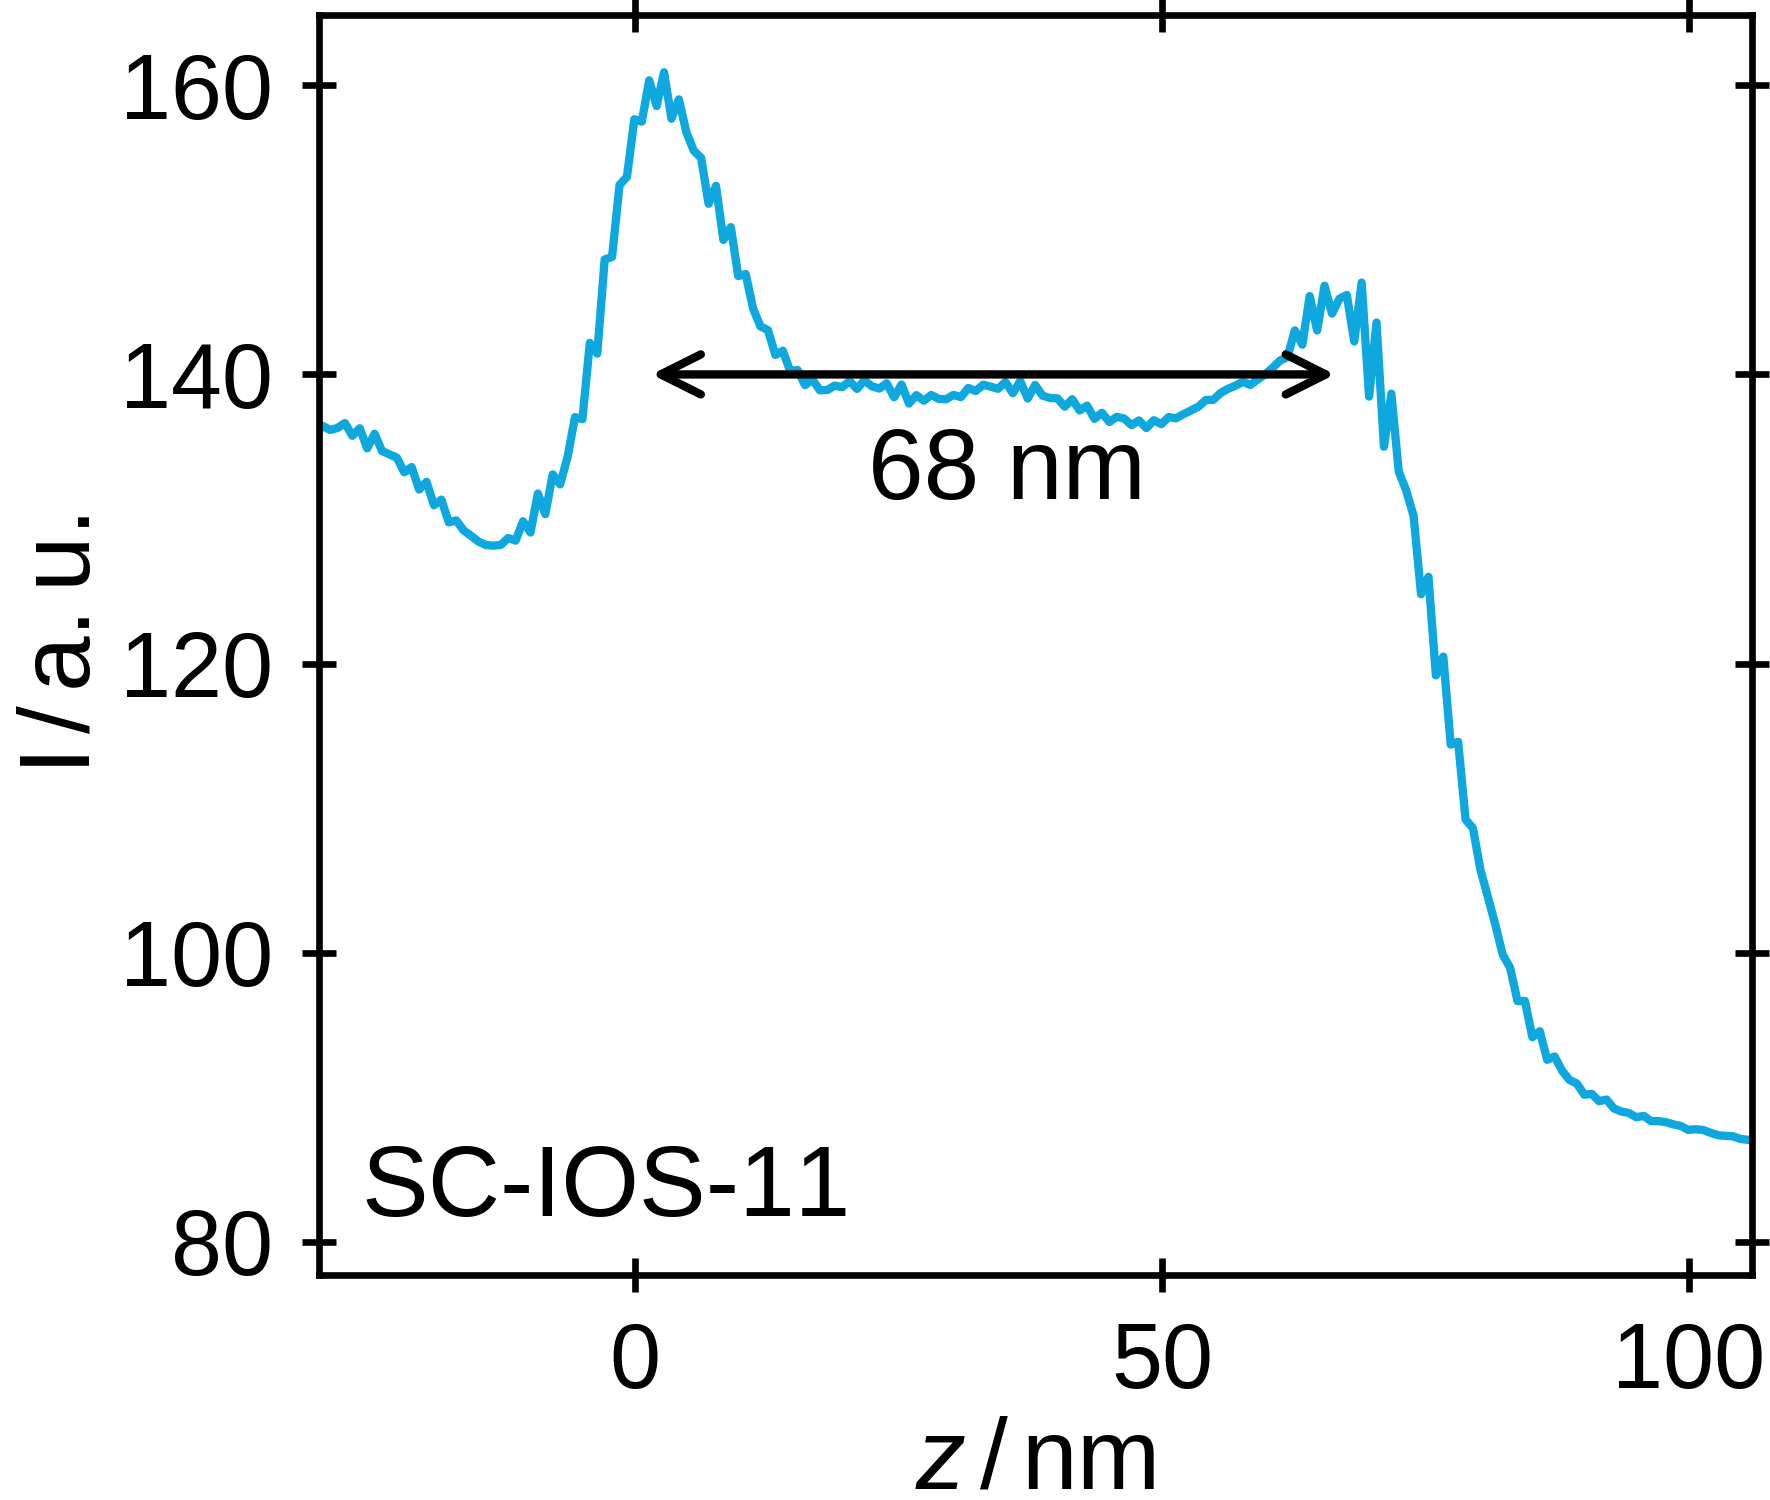
\includegraphics{looselyPackedNP_SEMprojection_SC-IOS-11}
  %   \caption{\label{fig:looselyPackedNP:nuclearStructure:semProjection}Projection of the pixel intensity along the vertical axis from the cross-sectional SEM shown in \reffig{fig:looselyPackedNP:nuclearStructure:sem}.}
  % \end{figure}
\end{document}